\documentclass[11pt,a4paper]{article}
\usepackage[margin=1in, headheight=14pt]{geometry}
\usepackage{amsfonts,amsmath,amssymb,suetterl}
\usepackage{lmodern}
\usepackage[T1]{fontenc}
\usepackage{fancyhdr}
\usepackage{float}
\usepackage[utf8]{inputenc}
\usepackage{fontawesome}
\usepackage{enumerate}
\usepackage{xcolor}
\usepackage{hyperref}
\usepackage{tikz}
\usepackage{nicefrac}
\usepackage{subcaption}
\usepackage{physics}
\usepackage{mathtools}
\usepackage{adjustbox}

\DeclareUnicodeCharacter{2212}{-}

\usepackage{mathrsfs}
\usepackage[nodisplayskipstretch]{setspace}

\setstretch{1.5}
\renewcommand{\footrulewidth}{0pt}

\pagestyle{fancy}
\fancyhead[R]{Problem Sheet 5 (Solutions)}
\fancyhead[L]{MA202: Differential Equations}

\parindent 0ex
\setlength{\parskip}{1em}
\raggedbottom

\begin{document}
	\begin{center}
		\textbf{Problem Sheet 5 - Solutions}
	\end{center}
	%
	\begin{enumerate}
		\item \textbf{(A)} The trajectories are solutions of the differential equation
		$$
		\frac{dy}{dx} = \frac{4x}{y},
		$$
		which can also be written as $4xdx - ydy = 0$. Integrating, we obtain
		$$
		4x^2 - y^2 = C.
		$$
		Hence the trajectories are hyperbolas (for $C \neq 0$) and the straight lines $y = \pm 2x$ (for $C = 0$).
		%
		\begin{figure}[H]
			\centering
			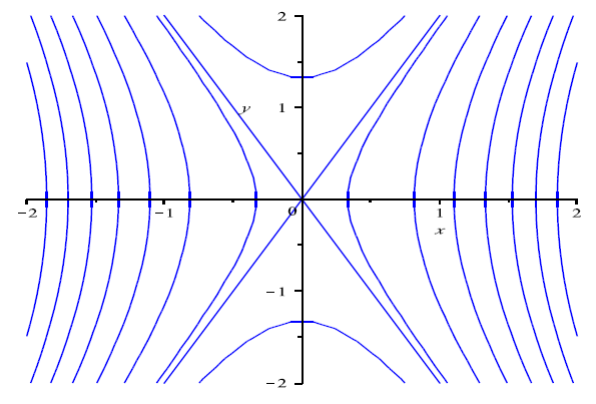
\includegraphics[width=0.45\textwidth]{figure/6_fig1.PNG}
			\caption{The phase trajectories for the system in Question 1A.}
		\end{figure}
		%
		Based on the differential equations, in the first quadrant both $x$ and $y$ are increasing, in the second quadrant $x$ is increasing and $y$ is decreasing, in the third quadrant both $x$ and $y$ are decreasing, and in the fourth quadrant $x$ is decreasing and $y$ is increasing (see Fig. 1).\\
		\textbf{(B)} The trajectories are solutions of the differential equation
		$$
		\frac{dy}{dx} = \frac{x+y}{x-y},
		$$
		which is homogeneous. Setting $y = xv(x)$, we obtain
		$$
		v + x\frac{dv}{dx} = \frac{x + xv}{x - xv}.
		$$
		that is,
		$$
		x\frac{dv}{dx} = \frac{1 + v^2}{1 - v}.
		$$
		The resulting ODE is separable, with solution
		$$
		\arctan v = \ln|x|\sqrt{1 + v^2}.
		$$
		%
		\begin{figure}[H]
			\centering
			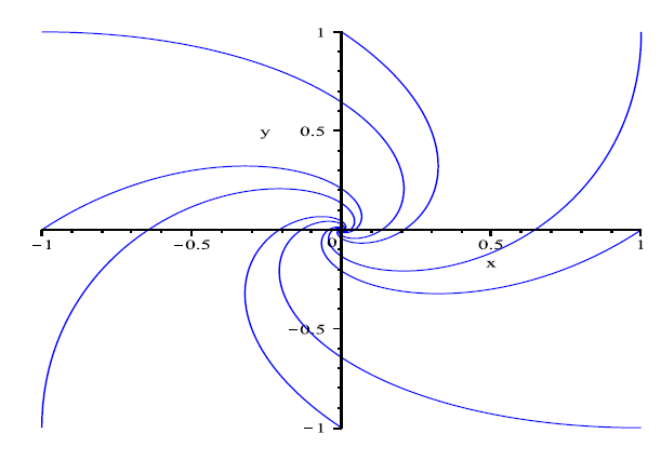
\includegraphics[width=0.45\textwidth]{figure/6_fig2.PNG}
			\caption{The phase trajectories for the system in Question 1B.}
		\end{figure}
		%
		Reverting back to the original variables, the trajectories are level curves of
		$$
		H(x,y) = \arctan(y/x) - \ln\sqrt{x^2 + y^2}.
		$$
		The origin is a stable spiral (Fig.2).\\
		\textbf{(C)} The trajectories are solutions of the differential equation
		$$
		\frac{dy}{dx} = \frac{y - 2xy}{-x + y + x^2},
		$$
		which can also be written as $(y - 2xy)dx + (x - y - x^2)dy = 0$. The resulting ODE is exact, with $H_x = y - 2xy$ and $H_y = x - y - x^2$. Integrating the first equation, we find that $H(x, y) = xy - x^2y + f(y)$. It follows that $H_y = x - x^2 + f^\prime(y)$. Comparing the two partial derivatives, we obtain $f(y) = -y^2/2 + c$. Hence
		$$
		H(x,y) = xy - x^2y - \frac{y^2}{2}.
		$$
		The associated direction field shows the direction of motion along the trajectories as depicted on Figure 3.
		%
		\begin{figure}[H]
			\centering
			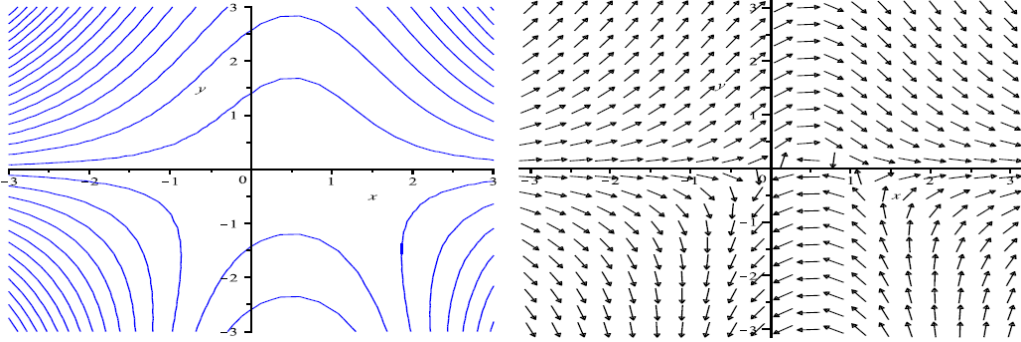
\includegraphics[width=0.85\textwidth]{figure/6_fig3.PNG}
			\caption{The phase trajectories (left) and the direction field (right) for the system in Question 1C.}
		\end{figure}
		%
		\item Let $C_0$ be the trajectory generated by the solution $x = \phi_0(t),\ y = \psi_0(t)$ with $\phi_0(t_0) = x_0,\ \psi_0(t_0) = y_0$ and let $C_1$ be the trajectory generated by the solution $x = \phi_1(t),\ y = \psi_1(t)$ with $\phi_1(t_1) = x_0,\ \psi_1(t_1) = y_0$.\\
		If we denote $\Phi(t) = \phi(t - s)$ and $\Psi(t) = \psi(t - s)$, we can write
		\begin{align*}
			\frac{d\Phi}{dt}(t) &= \frac{d\phi}{dt}(t-s) = F(\phi(t-s),\psi(t-s)) = F(\Phi(t), \Psi(t));\\
			\frac{d\Phi}{dt}(t) &= \frac{d\psi}{dt}(t-s) = G(\phi(t-s),\psi(t-s)) = G(\Phi(t), \Psi(t)).
		\end{align*}
		Therefore $\Phi_1(t) = \phi_1(t - (t_0 - t_1)),\ \Psi_1(t) = \psi_1(t - (t_0 - t_1))$ is a solution.\\
		Furthermore, $|phi_1(t_0) = \phi_1(t_1) = x_0$ and $\Psi_1(t_0) = y_0$. Then, by uniqueness, $\phi_0(t) = \Phi_1(t)$ and $\psi_0(t) = \Psi_1(t)$. Therefore, the trajectories are the same: $C_0 \equiv C_1$.
		\item From the existence and uniqueness theorem we know that if the two solutions $x = \phi(t)$ and $y = \psi(t)$ with $x = x_0$ and $y = y_0$ satisfy $\phi(a) = x_0$ and $\psi(a) = y_0$ with $x = x_0$ and $y = y_0$ at $t = a$, then these solutions are identical. Hence $\phi(t) = x_0$ and $\psi(t) = y_0$ for all $t$ contradicting the fact that the trajectory generated by $\phi(t)$ and $\psi(t)$ started at a noncritical point.
		\item \textbf{(A)} The critical points consist of the solution set of the equations
		\begin{align*}
			(3 + x)(y-x) &= 0;\\
			(4 - x)(y + x) &= 0.
		\end{align*}
		From the first equation, $x = -3$ or $y = x$. When $x = 3$, then $y = -3$ from the second equation. When $y = x$, the second equation gives $x = 4$ or $x = 0$. The critical points are at $(0, 0)$, $(4, 4)$ and $(-3, 3)$.\\
		We have $F(x, y) = (3 + x)(y - x)$ and $G(x, y) = (4 - x)(y + x)$. The Jacobian matrix of the vector field is
		$$
		J =
		\begin{pmatrix}
			F_x(x, y) & F_y(x, y)\\
			G_x(x, y) & G_y(x, y)
		\end{pmatrix} = 
		\begin{pmatrix}
			-3 - 2x + y & 3 + x\\
			4 - y - 2x & 4 - x
		\end{pmatrix}.
		$$
		At the origin, the coefficient matrix of the linearized system is
		$$
		J(0, 0) =
		\begin{pmatrix}
			-3 & 3\\
			-4 & 4
		\end{pmatrix}.
		$$
		with eigenvalues $r_1 = \sqrt{97}/2$ and $r_2 = 1/2 + \sqrt{97}/2$. The eigenvalues are real, with opposite sign. Hence the critical point is a saddle, which is unstable.\\
		At the point $(-3, 3)$, the coefficient matrix of the linearized system is
		$$
		J(0, 0) = 
		\begin{pmatrix}
			6 & 0\\
			7 & 7
		\end{pmatrix}
		$$,
		with eigenvalues $r_1 = 6$ and $r_2 = 7$. The eigenvalues are real, unequal and positive, hence the critical point is an unstable node.\\
		At the point $(4, 4)$, the coefficient matrix of the linearized system is
		$$
		J =
		\begin{pmatrix}
			-7 & 7\\
			-8 & 0
		\end{pmatrix},
		$$
		with complex conjugate eigenvalues $r_{1,2} = -7/2 \pm i5\sqrt{7}/2$. The critical point is a stable spiral, which is asymptotically stable.\\
		The nonlinear terms do not affect the stability and type of each critical point (the phase portrait of the system is shown in Fig. 4A).
		%
		\begin{figure}[H]
			\centering
			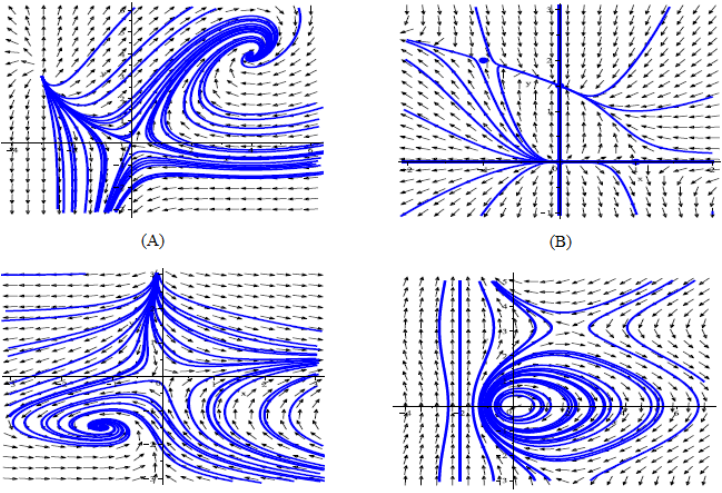
\includegraphics[width=0.85\textwidth]{figure/6_fig4.PNG}
			\caption{The phase trajectories for the systems in Question 4.}
		\end{figure}
		%
		\textbf{(B)} The critical points consist of the solution set of the equations $x(1 - x - y) = 0$ and $y(3 - x - 2y) = 0$. Solutions are $x = 0\, y = 0;\ x = 0,\ 3 - 2y = 0$ i.e. $y = 3/2;\ y = 0,\ 1 - x = 0$ i.e. $x = 1$; and $1 - x - y = 0,\ 3 - x - 2y = 0$ which give $x = -1,\ y = 2$. Thus we found the four critical points $(0, 0),\ (0, 3/2),\ (1, 0),\ (-1, 2)$.\\
		Here, we have $F(x, y) = x - x^2 - xy$ and $G(x, y) = 3y - xy - 2y^2$. Therefore, the Jacobian matrix for this system is
		$$
		\begin{pmatrix}
			F_x(x,y) & F_y(x, y)\\
			G_x(x, y) & G_y(x, y)
		\end{pmatrix} =
		\begin{pmatrix}
			1 - 2x - y & -x\\
			-y & 3 - x - 4y
		\end{pmatrix}.
		$$
		Therefore, near the critical point $(0, 0)$, the Jacobian matrix is
		$$
		J(0, 0) =
		\begin{pmatrix}
			1 & 0\\
			0 & 3
		\end{pmatrix}
		$$
		and the corresponding linear system near $(0, 0)$ is
		$$
		\frac{d}{dt}
		\begin{pmatrix}
			u\\
			v
		\end{pmatrix} =
		\begin{pmatrix}
			1 & 0\\
			0 & 3
		\end{pmatrix}
		\begin{pmatrix}
			u\\
			v
		\end{pmatrix}
		$$
		Near the critical point $(0, 3/2)$, the Jacobian matrix is
		$$
		J(0, 3/2) =
		\begin{pmatrix}
			-1/2 & 0\\
			-3/2 & -3
		\end{pmatrix}
		$$
		and the corresponding linear system near $(0, 3/2)$ is
		$$
		\frac{d}{dt}
		\begin{pmatrix}
			u\\
			v
		\end{pmatrix} =
		\begin{pmatrix}
			-1/2 & 0\\
			-3/2 & -3
		\end{pmatrix}
		\begin{pmatrix}
			u\\
			v
		\end{pmatrix}
		$$
		where $u = x$ and $v = y - 3/2$. Near the critical point $(1, 0)$, the Jacobian matrix is
		$$
		J(1, 0) =
		\begin{pmatrix}
			-1 & -1\\
			0 & 2
		\end{pmatrix}
		$$
		and the corresponding linear system near $(1, 0)$ is
		$$
		\frac{d}{dt} 
		\begin{pmatrix}
			u\\
			v
		\end{pmatrix} =
		\begin{pmatrix}
			-1 & -1\\
			0 & 2
		\end{pmatrix}
		\begin{pmatrix}
			u\\
			v
		\end{pmatrix}
		$$
		where $u = x - 1$ and $v = y$. Near the critical point $(-1, 2)$, the Jacobian matrix is
		$$
		J(-1, 2) =
		\begin{pmatrix}
			1 & 1\\
			-2 & 4
		\end{pmatrix}
		$$
		and the corresponding linear system near $(-1, 2)$ is
		$$
		\frac{d}{dt}
		\begin{pmatrix}
			u\\
			v
		\end{pmatrix} =
		\begin{pmatrix}
			1 & 1\\
			-2 & 4
		\end{pmatrix}
		\begin{pmatrix}
			u\\
			v
		\end{pmatrix}
		$$
		where $u = x + 1$ and $v = y - 2$.\\
		The eigenvalues of the linear system near $(0, 0)$ are $\lambda = 1,\ 3$. From this, we can conclude that $(0, 0)$ is an unstable node for the nonlinear system. The eigenvalues of the linear system near $(0, 3/2)$ are $\lambda = -1/2,\ -3$. From this, we can conclude that $(0, 3/2)$ is an asymptotically stable node for the nonlinear system. The eigenvalues of the linear system near $(1, 0)$ are $\lambda = -1,\ 2$. From this, we can conclude that $(1, 0)$ is a saddle point for the nonlinear system. The eigenvalues of the linear system near $(-1, 2)$ are $\lambda = (-3 \pm \sqrt{17})/2$. From this, we can conclude that $(-1, 2)$ is an unstable saddle point for the nonlinear system. The phase portrait is depicted on Fig. 4B.\\
		\textbf{(C)} The critical points are solutions of the equations
		\begin{align*}
			2x + y + xy^3 &= 0\\
			x - 2y - xy &= 0
		\end{align*}
		Substitution of $y = x/(x + 2)$ into the first equation results in
		$$
		3x^4 + 13x^3 + 28x^2 + 20x = 0.
		$$
		One root of the resulting equation is $x = 0$. The only other real root of the equation is
		$$
		x = \frac{1}{9}\left[(287 + 18\sqrt{2019})^{\nicefrac{1}{3}} - 83(287 + 18\sqrt{2019})^{-\nicefrac{1}{3}} - 13\right].
		$$
		Hence the critical points are $(0, 0)$ and $(-1.19345\ldots,\ -1.4797\ldots)$.\\
		For the given functions $F(x, y) = 2x + y + xy^3$ and $G(x, y) = x - 2y - xy$ the Jacobian matrix of the vector field is
		$$
		\begin{pmatrix}
			F_x(x, y) & F_y(x, y)\\
			G_x(x, y) & G_y(x, y)
		\end{pmatrix} =
		\begin{pmatrix}
			2 + y^3 & 1 + 3xy^2\\
			1 - y & 3 - 2 - x
		\end{pmatrix}.
		$$
		At the origin, the coefficient matrix of the linearized system is
		$$
		J(0, 0) =
		\begin{pmatrix}
			2 & 1\\
			1 & -2
		\end{pmatrix}
		$$
		with eigenvalues $r_1 = \sqrt{5}$ and $r_2 = -\sqrt{5}$. The eigenvalues are real and of opposite sign. Hence the critical point is a saddle, which is unstable.\\
		At the point $(-1.19345\ldots, -1.4797\ldots)$, the coefficient matrix of the linearized system is
		$$
		J(-1.19345, -1.4797) = 
		\begin{pmatrix}
			-1.2399 & -6.8393\\
			2.4797 & -0.8065
		\end{pmatrix},
		$$
		with complex conjugate eigenvalues $r_{1,2} = -1.0232 \pm 4.1125i$. The critical point is a stable spiral, which is asymptotically stable. In both cases, the nonlinear terms do not affect the stability and type of the critical point. The phase portrait is depicted on Fig. 4C.\\
		\textbf{(D)} The critical points are given by the solution set of the equations
		\begin{align*}
			(2 + x)\sin y &= 0\\
			1 - x - \cos y &= 0.
		\end{align*}
		If $x = -2$, then we must have $\cos y = 3$, which is impossible (for real $y$). Therefore $\sin y = 0$, which implies that $y = n\pi,\ n \in \mathbb{Z}$. Based on the second equation,
		$$
		x = 1 - \cos n\pi
		$$
		It follows that the critical points are located at $(0, 2k\pi)$ and $(2, (2k + 1)\pi)$, where $k \in \mathbb{Z}$. Given that $F(x, y) = (2 + x) \sin y$ and $G(x, y) = 1 - x - \cos y$, the Jacobian matrix of the vector field is
		$$
		\begin{pmatrix}
			F_x(x, y) & F_y(x, y)\\
			G_x(x, y) & G_y(x, y)
		\end{pmatrix} =
		\begin{pmatrix}
			\sin y & (2+x)\cos y\\
			-1 & \sin y
		\end{pmatrix}.
		$$
		At the critical points $(0, 2k\pi)$, the coefficient matrix of the linearized system is
		$$
		J(0, 2k\pi) =
		\begin{pmatrix}
			0 & 2\\
			-1 & 0
		\end{pmatrix}
		$$
		with purely imaginary eigenvalues $r_{1,2} = \pm\sqrt{2}i$. The critical points of the associated linear systems are centers, which are stable (see Theorem 9.3.2 in the main Textbook).\\
		Note that Theorem 9.3.2 does not provide a definite conclusion regarding the relation between the nature of the critical points of the nonlinear systems and their corresponding linearisations.\\
		At the points $(2, (2k + 1)\pi)$, the coefficient matrix of the linearized system is
		$$
		J[2, (2k + 1)\pi] =
		\begin{pmatrix}
			0 & -4\\
			-1 & 0
		\end{pmatrix},
		$$
		with eigenvalues $r_1 = 2$ and $r_2 = -2$. The eigenvalues are real, with opposite sign. Hence the critical points of the associated linear systems are saddles, which are unstable.\\
		As asserted in Theorem 9.3.2 in the main Textbook, the trajectories near the critical points $(2,(2k+1)\pi)$ resemble those near a saddle. Upon closer examination, the critical points $(0, 2k\pi)$ are indeed centers (See Fig. 4D).
		\item \textbf{(A)} The critical points are the solutions of the system
		\begin{align*}
			x(a - \sigma x - \alpha y) &= 0\\
			y(-c + \gamma x) &= 0
		\end{align*}
		If $x = 0$, then $y = 0$. If $y = 0$, then $x = a/\sigma$. The third solution is found by substituting $x = c/\gamma$ into the first equation. This implies that $y = a/\alpha - \sigma c/(\gamma\alpha)$.\\
		So the critical points are $(0, 0),\ \left(\frac{a}{\sigma}, 0\right)$ and $\left(\frac{c}{\gamma}, \frac{a}{\alpha}-\frac{\sigma c}{\gamma \alpha}\right)$. When $\sigma$ is increasing, the critical point $\left(\frac{a}{\sigma}, 0\right)$ moves to the left and the critical point $\left(\frac{c}{\gamma}, \frac{a}{\alpha}-\frac{\sigma c}{\gamma \alpha}\right)$ moves down. The assumption $a > \sigma c/\gamma$ is necessary for the third critical point to be in the first quadrant. (When $a = \sigma c/\gamma$, then the two nonzero critical points coincide.)\\
		\textbf{(B)} The Jacobian of the system is
		$$
		J =
		\begin{pmatrix}
			a - 2\sigma x - \alpha y & -\alpha x\\
			\gamma y & -c + \gamma x
		\end{pmatrix}.
		$$
		This implies that at the origin
		$$
		J(0, 0) =
		\begin{pmatrix}
			a & 0\\
			0 & -c
		\end{pmatrix},
		$$
		which implies that the origin is a saddle point. ($a > 0$ and $c > 0$ by our assumption.) At the critical point $\left(\frac{a}{\sigma}, 0\right)$ we have
		$$
		J\left(\frac{a}{\sigma}, 0\right) =
		\begin{pmatrix}
			-a & -\frac{\alpha a}{\sigma}\\
			0 & -c + \frac{\gamma a}{\sigma}
		\end{pmatrix},
		$$
		which implies that this critical point is also a saddle as long as our assumption $a > \sigma c/\gamma$ is valid.\\
		At the critical point $\left(\frac{c}{\gamma}, \frac{a}{\alpha}-\frac{\sigma c}{\gamma \alpha}\right)$:
		$$
		J\left(\frac{c}{\gamma}, \frac{a}{\alpha}-\frac{\sigma c}{\gamma \alpha}\right) =
		\begin{pmatrix}
			-\frac{
				
			\sigma c}{\gamma} & -\frac{\alpha c}{\gamma}\\
			\frac{\gamma a}{\alpha} - \frac{\sigma c}{\alpha} & 0
		\end{pmatrix}.
		$$
		The eigenvalues of the matrix are
		$$
		\frac{-c\sigma \pm \sqrt{c^2\sigma^2 + 4c^2\gamma \sigma - 4ac\gamma^2}}{2\gamma}.
		$$
		\textbf{(C)} We set the discriminant equal to zero and find that the greater solution is
		$$
		\sigma_1 = -2\gamma + \frac{2\gamma\sqrt{ac + c^2}}{c}.
		$$
		First note that $\sigma_1 > 0$, since $\sqrt{ac + c^2} > c$. Next we note that $\sigma_1 < a\gamma/c$. Since
		$$
		\sqrt{ac + c^2}<\sqrt{\frac{a^2}{4} + ac + c^2} = \frac{a}{2} + c,
		$$
		we see that
		$$
		\sigma_1 = -2\gamma + \frac{2\gamma \sqrt{ac + c^2}}{c} < -2\gamma + \frac{2\gamma}{c}\left(\frac{a}{2}+c\right) = -2\gamma + \frac{a\gamma}{c} + 2\gamma = \frac{a\gamma}{c}.
		$$
		For $0 < \sigma < \sigma_1$, the eigenvalues will be complex conjugates with negative real part, so the critical point will be an asymptotically stable spiral point. For $\sigma = \sigma_1$, the eigenvalues will be repeated and negative, so the critical point will be an asymptotically stable spiral point or node. For $\sigma_1 < \sigma < ac/\gamma$, the eigenvalues will be distinct and negative, so the critical point will be an asymptotically stable node.\\
		\textbf{(D)} Since the third critical point is asymptotically stable for $0 < \sigma < ac/\gamma$, and the other critical points are saddle points, the populations will coexist for all such values of $\sigma$.
		\item \textbf{(A)} We consider the function $V(x, y) = ax^2 + cy^2$. The rate of change of $V$ along any trajectory is
		\begin{align*}
			\dot{V} 
			&= V_x\frac{dx}{dt} + V_x\frac{dy}{dt} = 2ax(-x^3 + 2xy^2) + 2cy(-2x^2y - y^3)\\
			&= -(2ax^4 + 4(c-a)x^2y^2 + 2cy^4).
		\end{align*}
		If we choose $a$ and $c$ be any positive real numbers with $c \geq a$, then $\dot{V} (x, y)$ is negative definite. By definition $V$ is positive definite. It follows from Theorem 9.6.1 in the main Textbook that the origin is an asymptotically stable critical point.\\
		\textbf{(B)} Again we consider the function $V (x, y) = ax^2 + cy^2$. The rate of change of $V$ along any trajectory is
		\begin{align*}
			\dot{V}
			&= V_x\frac{dx}{dt} + V_y\frac{dy}{dt} = 2ax(-2x^3 + 2y^3) + 2cy(-2xy^2)\\
			&= -4ax^4 + 4(a-c)xy^3.
		\end{align*}
		If we choose $a$ and $c$ to be any positive real numbers with $a = c$, then $\dot{V} (x, y) = -4ax^4 \leq 0$ in any neighborhood containing the origin and thus $\dot{V}$ is negative semi-definite. By definition V is positive definite. It follows from Theorem 9.6.1 in the main Textbook that the origin is a stable critical point. However, the origin may still be asymptotically stable although the $V(x, y)$ used here is not sufficient to prove that.\\
		\textbf{(C)}  Given $V(x, y) = ax^2 + cy^2$, the rate of change of $V$ along any trajectory is
		\begin{align*}
			\dot{V}
			&= V_x \frac{dx}{dt} + V_y\frac{dy}{dt} = 2ax(2x^3 - y^3) + 2cy(2xy^2 + 4x^2y + 2y^3)\\
			&= 4ax^4 + (4c - 2a)xy^3 + 8cx^2y^2 + 4cy^4.
		\end{align*}
		Setting $a = 2c$,
		$$
		\dot{V} = 8cx^4 + 8cx^2y^2 + 4cy^4 \geq 8cx^4 + 4cy^4.
		$$
		As long as $a = 2c > 0$, the function $V (x, y)$ is positive definite and $\dot{V} (x, y)$ is also positive definite. It follows from Theorem 9.6.2 in the main Textbook that $(0, 0)$ is an unstable critical point.
		\item Given $V(x, y) = c(x^2 + y^2)$, the rate of change of $V$ along any trajectory is
		\begin{align*}
			\dot{V}
			&= V_x\frac{dx}{dt} + V_y\frac{dy}{dt} = 2cx[y-xf(x,y)] + 2cy[-x-yf(x,y)]\\
			&= -2c(x^2 + y^2)f(x,y).
		\end{align*}
		If $c > 0$, then $V (x, y)$ is positive definite. Furthermore, if $f(x, y)$ is positive in some neighborhood of the origin, then $\dot{V}(x, y)$ is negative definite. Theorem 9.6.1 in the main Textbook asserts that the origin is an asymptotically stable critical point. On the other hand, if $f(x, y)$ is negative in some neighborhood of the origin, then $V(x, y)$ and $\dot{V} (x, y)$ are both positive definite. It follows from Theorem 9.6.2 in the main Textbook that the origin is an unstable critical point.
		\item \textbf{(A)} Note that $r = 2,\ \theta = t + t_0$ satisfy the two equations for all $t$ and is thus a periodic solution. We notice that for $0 < r < 2,\ dr/dt > 0$, while for $r > 2,\ dr/dt < 0$. Therefore, $r = 0$ is an unstable critical point, while $r = 2$ is an asymptotically stable critical point (for the $dr/dt$ equation). Thus a limit cycle is given by $r = 2,\ \theta = t + t_0$, which is asymptotically stable.\\
		\textbf{(B)} The critical points of the ODE
		$$
		\frac{dr}{dt} = r(r - 2)(r - 3)
		$$
		are given by $r_1 = 0,\ r_2 = 2$ and $r_3 = 3$. Note that $dr/dt > 0$ for $0 < r < 2$ and $r > 3$; $dr/dt < 0$ for $2 < r < 3$.\\
		The value $r = 0$ corresponds to an unstable critical point. The critical point $r_2 = 2$ is asymptotically stable, whereas the critical point $r_3 = 3$ is unstable. Since the critical values are isolated, a limit cycle is given by
		$$
		r = 2,\quad \theta = t + t_0,
		$$
		which is asymptotically stable. Another periodic solution is found to be
		$$
		r = 3,\quad \theta = t + t_0
		$$
		which is unstable.\\
		\textbf{(C)} The critical points of the ODE
		$$
		\frac{dr}{dt} = \sin \pi r
		$$
		are given by $r = n,\ n = 0,\ 1,\ 2,\ \ldots $. Based on the sign of $r_0$ in the neighborhood of each critical value, the critical points $r = 2k,\ k = 0,\ 1,\ 2,\ \ldots$ correspond to unstable periodic solutions, with $\theta = t + t_0$. The critical points $r = 2k + 1,\ k = 0,\ 1,\ 2,\ \ldots$ correspond to stable limit cycles, with $\theta = t + t_0$. The solution $r = 0$ represents an unstable critical point.
		\item If we introduce polar coordinates $x = r \cos \theta,\ y = r sin \theta$, by a direct computation we find that
		\begin{align*}
			y\frac{dx}{dt} - x\frac{dy}{dt}
			&= r\sin \theta \left[\cos \theta\frac{dr}{dt} - r\sin \theta\frac{d\theta}{dt}\right] - r\cos \theta\left[\sin \theta\frac{dr}{dt} + r\cos \theta \frac{d\theta}{dt}\right]\\
			&=-r^2\sin^2\theta\frac{d\theta}{dt} - r^2\cos^2\theta\frac{d\theta}{dt} = -r^2\frac{d\theta}{dt}.
		\end{align*}
		Since $r^2 = x^2 + y^2$, we have
		$$
		r\frac{dr}{dt} = x\frac{dx}{dt} + y\frac{dy}{dt}.
		$$
		Thus
		$$
		r\frac{dr}{dt} = \frac{x^2f(r)}{r} + \frac{y^2f(r)}{r} = \frac{r^2f(r)}{r} = rf(r).
		$$
		Therefore, $rdr/dt = rf(r)$, which implies $dr/dt = f(r)$. Therefore, we have periodic solutions corresponding to the zeros of $f(r)$. To find the direction of motion on the closed trajectories, we need to find:
		$$
		-r^2\frac{d\theta}{dt} = y\frac{dx}{dt} - x\frac{dy}{dt} = -y^2 + \frac{xyf(r)}{r} - x^2 - \frac{xyf(r)}{r} = -x^2 - y^2 = -r^2.
		$$
		Therefore, $d\theta/dt = 1$, which implies $\theta = t + t_0$. Therefore, the closed trajectories will move in the counter-clockwise direction.\\
		\textbf{(B)} By part (A), we know the periodic solutions will be given by the zeros of $f$. The zeros are $r = 0;\ 1;\ 2;\ 4$. Using the fact that $dr/dt = f(r)$, we see that $dr/dt > 0$ if $0 < r < 1$ and $r > 4$ and $dr/dt < 0$ if $1 < r < 2$ and $2 < r < 4$. Therefore, $r = 0$ is unstable, $r = 1$ is asymptotically stable, $r = 2$ is semi-stable, and $r = 4$ is unstable.\\
		We conclude that there is an asymptotically stable limit cycle at $r = 1$ with $\theta = t + t_0$, a semi-stable limit cycle at $r = 2$ with $\theta = t + t_0$ and an unstable periodic solution at $r = 4$ with $\theta = t + t_0$.
		\item \textbf{(A)} Using the fact that
		$$
		r\frac{dr}{dt} = x\frac{dx}{dt} + y\frac{dy}{dt},
		$$
		we have
		$$
		r\frac{dr}{dt} = xy + \frac{x^2}{\sqrt{x^2 + y^2}}(x^2 + y^2 - 3) - xy + \frac{y^2}{\sqrt{x^2 + y^2}}(x^2 + y^2 - 3) = r(r^2 - 3).
		$$
		Therefore, $\frac{dr}{dt} = r^2 - 3$, so we have one critical point at $r = \sqrt{3}$. We see that $\frac{dr}{dt} > 0$ if $r > \sqrt{3}$ and $\frac{dr}{dt} < 0$ if $r< \sqrt
		3$. Therefore, $r = \sqrt{3}$ is an unstable periodic solution. To find the direction of motion on the closed trajectories, we use the fact that
		$$
		-r^2\frac{d\theta}{dt} = y\frac{dx}{dt} - x\frac{dy}{dt}.
		$$
		Therefore, here we have
		$$
		-r^2\frac{d\theta}{dt} = y^2 + x^2 = r^2,
		$$
		so, $\frac{d\theta}{dt} = -1$, which implies $\theta = -t + t_0$.\\
		\textbf{(B)} Given $F(x, y) = a_{11}x + a_{12}y$ and $G(x, y) = a_{21}x + a_{22}y$, it follows that
		$$
		F_x + G_y = a_{11} + a_{22}.
		$$
		Based on the hypothesis, $F_x + G_y$ is either positive or negative on the entire plane. By Theorem 9.7.2 in the main Textbook, the system cannot have a nontrivial periodic solution.\\
		\textbf{(C)} Given that $F(x, y) = -3x - 3y - xy^2$ and $G(x, y) = 2y + x^3 - x^2y$, we have
		$$
		F_x + G_y = -1 - x^2 - y^2.
		$$
		Since $F_x + G_y < 0$ on the entire plane, Theorem 9.7.2 in the main Textbook asserts that the system cannot have a nontrivial periodic solution.
		\item \textbf{(A)} The critical points are solutions of the algebraic system
		\begin{align*}
			\mu x + y - x(x^2 + y^2) &= 0\\
			-x + \mu y - y(x^2 + y^2) &= 0
		\end{align*}
		Multiply the first equation by $y$ and the second equation by $x$ to obtain
		\begin{align*}
			\mu x y + y^2 - xy(x^2 + y^2) &= 0\\
			-x^2 + \mu xy - xy(x^2 + y^2) &= 0.
		\end{align*}
		Multiply the first equation by y and the second equation by x to obtain
		$$
		x^2 + y^2 = 0
		$$
		which is satisfied only for $x = y = 0$.\\
		\textbf{(B)} The Jacobian matrix of the vector field is
		$$
		J =
		\begin{pmatrix}
			\mu - 3x^2 - y^2 & 1 - 2xy\\
			-1 -2xy & \mu - x^2 -3y^2
		\end{pmatrix}.
		$$
		At the critical point $(0, 0)$, the coefficient matrix of the linearized system is
		$$
		J(0, 0) =
		\begin{pmatrix}
			\mu & 1\\
			-1 & \mu
		\end{pmatrix},
		$$
		resulting in the linear system
		\begin{align*}
			x^\prime &= \mu x + y\\
			y^\prime &= -x + \mu y.
		\end{align*}
		The characteristic equation for the coefficient matrix is $\lambda^2 - 2\mu \lambda + \mu^2 + 1 = 0$, with solutions
		$$
		\lambda = \mu \pm i.
		$$
		For $\mu < 0$, the origin is a stable spiral. When $\mu = 0$, the origin is a center. For $\mu > 0$, the origin is an unstable spiral.\\
		\textbf{(C)} Introduce polar coordinates $r$ and $\theta$, so that $x = r \cos \theta$ and $y = r \sin \theta$ for $r \geq 0$. Multiply the first equation of the original nonlinear system by $x$ and the second equation by $y$ to obtain
		\begin{align*}
			xx^\prime &= \mu x^2 + xy - x^2(x^2 + y^2),\\
			yy^\prime &= -xy + \mu y^2 - y^2(x^2 + y^2).
		\end{align*}
		Addition of the two equations results in
		$$
		xx^\prime + yy^\prime = \mu(x^2 + y^2) - (x^2 + y^2)^2.
		$$
		Since $r^2 = x^2 + y^2$ and $rr^\prime = xx^\prime + yy^\prime$, it follows that $rr^\prime = \mu r^2 - r^4$ and
		$$
		\frac{dr}{dt} = \mu r - r^3
		$$
		for $r > 0$. Multiply the first equation of the original nonlinear system by $y$ and the second equation by $x$, the difference of the two equations results in
		$$
		yx^\prime - xy^\prime = x^2 + y^2.
		$$
		Since $yx^\prime - xy^\prime = -r^2\theta^\prime$, the above equation reduces to
		$$
		\frac{d\theta}{dt} = -1.
		$$
		\textbf{(D)}  From $r^\prime = r(\mu - r^2)$ and $\theta^\prime = -1$, it follows that one solution of the system is given by
		$$
		r = \sqrt{\mu},\quad \text{and}\quad \theta = -t + t_0,
		$$
		valid for $\mu > 0$. This corresponds to a periodic solution with a circular trajectory. Since $r \geq 0$, observe that
		$$
		\frac{dr}{dt} = 
		\begin{cases}
			r(\mu - r^2) < 0 \quad \text{for} \quad r > \sqrt{\mu},\\
			r(\mu - r^2) > 0 \quad \text{for} \quad \sqrt{\mu} > r > 0.
		\end{cases}
		$$
		Hence solutions with initial condition $r(0) \neq \sqrt{\mu}$ are attracted to the limit cycle.
		\item \textbf{(A)} By a direct computation:
		\begin{align*}
			\frac{dV}{dt}
			&= \frac{\partial V}{\partial x} \frac{dx}{dt} + \frac{\partial V}{\partial y}\frac{dy}{dt} + \frac{\partial V}{\partial z}\frac{dz}{dt}2rx\frac{dx}{dt} + 2\sigma y\frac{dx}{dt} + 2\sigma(z-2r)\frac{dz}{dt}\\
			&= 2\sigma rx(-x + y) + 2\sigma y(rx - y - xz) + 2\sigma(z-2r)(-bz + xy)\\
			&= -2\sigma rx^2 - 2\sigma y^2 - 2\sigma bz^2 + 4\sigma rbz = -2\sigma(rx^2 + y^2 + bz^2 - 2rbz)\\
			&= -2\sigma [rx^2 + y^2 + b(z - r)^2 - br^2].
		\end{align*}
		\textbf{(B)}  From the proof of Theorem 9.6.1 in the main Textbook, we find that we need to show that $\dot{V}$, as found in part (A), is always negative as it crosses $V(x, y, z) = c$.\footnote{Actually, we need to use the extension of Theorem 9.6.1 to three equations, but the proof is very similar using the vector calculus approach.
		} From part (A) we see that $\dot{V} < 0$ whenever $rx^2 + y^2 + b(z - r)^2 > br^2$, which holds if $(x, y, z)$ lies outside the ellipsoid
		\begin{equation}
			\frac{x^2}{br} + \frac{y^2}{br^2} + \frac{(z-r)^2}{r^2} = 1.
		\end{equation}
		Thus we need to choose c such that $V = c$ lies outside Eq.(1). Writing $V = c$ in the form of Eq.(1) we obtain the ellipsoid
		\begin{equation}
			\frac{x^2}{(c/r)} + \frac{y^2}{(c/\sigma)} + \frac{(z-2r)^2}{(c/\sigma)} = 1.
		\end{equation}
		Now let $M = \max (\sqrt{br},\ r\sqrt{b},\ r)$, then the ellipsoid (1) is contained inside the sphere $\sum_1$:
		$$
		\textstyle{\sum_1}:\ \frac{x^2}{M^2} + \frac{y^2}{M^2} + \frac{(z-r)^2}{M^2} = 1,
		$$
		Let $\sum_2$ be a sphere centered at $(0, 0, 2r)$ with radius $M + r$:
		$$
		\textstyle{\sum_2}:\ \frac{x^2}{(M + r)^2} + \frac{y^2}{(M+r)^2} + \frac{(z - 2r)^2}{(M+r)^2} = 1,
		$$
		then $\sum_1$ is contained in $\sum_2$. Thus, if we choose $c$, in Eq.(2), such that $c/r > (M +r)^2$ and $c/\sigma > (M + r)^2$, then $\dot{V} < 0$ as the trajectory crosses $V (x, y, z) = c$.\\
		\textit{Note that this is a sufficient condition and there may be many other better choices using different techniques.}\\
		\textbf{(C)} With the given values we obtain $c \approx 33 450.7$.
	\end{enumerate}
\end{document}